
\let\negmedspace\undefined
\let\negthickspace\undefined
\documentclass[journal,12pt,twocolumn]{IEEEtran}
\usepackage{cite}
\usepackage{amsmath,amssymb,amsfonts,amsthm}
\usepackage{algorithmic}
\usepackage{graphicx}
\usepackage{textcomp}
\usepackage{xcolor}
\usepackage{txfonts}
\usepackage{listings}
\usepackage{enumitem}
\usepackage{mathtools}
\usepackage{gensymb}
\usepackage[breaklinks=true]{hyperref}
\usepackage{tkz-euclide} % loads  TikZ and tkz-base
\usepackage{listings}

\begin{document}


\vspace{3cm}

\title{
%	\logo{
AI5030 - Hardware Assignment\\
Random number generation using Shift Registers%	}
}
\author{ Samuktha V. (AI23MTECH02004)

	\thanks{*The author is with the Department
		of Dept. of AI, Indian Institute of Technology, Hyderabad
		502285 India e-mail:  ai23mtech02004@iith.ac.in. All content in this manual is released under GNU GPL.  Free and open source.}
}

% make the title area
\maketitle

\newpage
\textbf{\emph{Aim:} To generate number in random order using shift registers}
\newline

\section{Components }
\begin{table}[htbp]
	\label{tab:Hardware_Assignment}
	\begin{tabular}{|l|l|l|}\hline
	Component	&Value &Quantity\\ \hline
	Breadboard & &1 \\ \hline
	Seven Segment Diplay &Common Anode &1 \\ \hline
	Decoder &7447 &1 \\ \hline
	Flip Flop &7474 &2 \\ \hline
	X-OR Gate &7486 &1 \\ \hline
	555 IC & &1 \\ \hline
	Resistor &1 K$\Omega$ &1 \\ \hline
	Capacitor &100 nF &1 \\ \hline
	Capacitor &10 nF &1 \\ \hline
	Jumper Wires & & \\ \hline
\end{tabular}

	\caption{List of Components}
\end{table}



\section{Procedure}
\begin{enumerate}[label=(\roman*)]
	\item The 555 timer circuit is used to generate the clock output for the flipflops.
	\item The Clock output of 555 timer circuit is given to the clock signal of D-Flip flops.
	\item The circuit for generating random numbers is designed with shift registers using  4 D-Flip flops (i.e., two 7474 ICs).
	\item The XOR gate (7486 IC) is connected.
	\item The decoder (7447 IC) is connected and its A,B,C,D is connected to $Q_0$,$Q_1$,$Q_2$,$Q_3$ respectively.
	\item To visualise the output the seven segment display is connected to the decoder (7447 IC).
\end{enumerate}

\textbf{Conclusion:} 
The project's primary objective of generating random numbers with uniform probability distribution is accomplished with the help of Flipflops acting as counters.
One application of the above project is playing an audio playlist in random order which is accomplished as the second part of the project as a Software assignment.
\begin{figure}[h]
    \centering
    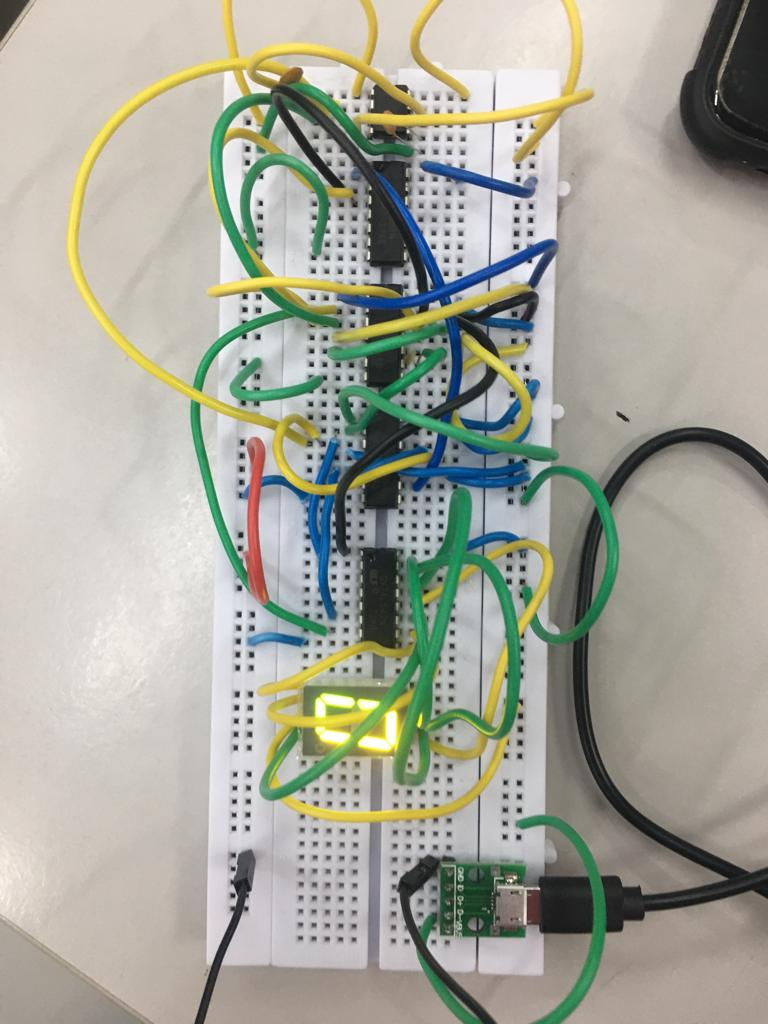
\includegraphics[scale=0.3]{cir.jpeg}
    \caption{Circuit displaying output}
    \label{fig:my_label}
\end{figure}
\end{document}
